\vspace{-0.1cm}
\section{Introduction}
\label{sec:introduction}

Aligning Large Language Models (LLMs) with human preferences is paramount for their safe and effective deployment, with Reinforcement Learning from Human Feedback (RLHF) and its reliance on reward models (RMs) being the dominant paradigm \citep{christiano2017deep, ouyang2022training, bai2022training, schulman2017proximal, shao2024deepseekmath, rafailov2024direct}. The fidelity of these RMs is critical, as flaws directly propagate to the aligned policy \citep{casper2023open}. 

However, standard RM training faces a significant challenge: \textit{reward hacking} \citep{gao2023scaling, skalse2022defining}. RMs often learn to assign high scores based on superficial or spurious attributes—such as response length \citep{singhal2023long}, specific formatting patterns \citep{zhang2024lists}, or stylistic quirks—because these features are statistically correlated with preferred responses in the training data. This occurs because standard training objectives do not explicitly require the RM to disentangle the true \textit{causal} drivers of response quality (e.g., factuality, relevance) from these spurious correlates, leading to brittle RMs and misaligned policies \citep{shen2023trickle, eisenstein2023helping}.



Recent efforts for RM robustness have explored various avenues. Some focus on consistency checks against meaning-preserving transformations \citep{wu2025rewordbench}, while others employ data augmentations, such as using non-contextual or query-independent comparisons to reduce spuriousness \citep{liu2024rrm}. 

\begin{wrapfigure}{r}{0.52\textwidth}
    \vspace{-0.1in}
    % \begin{figure}[!t]
    \centering
    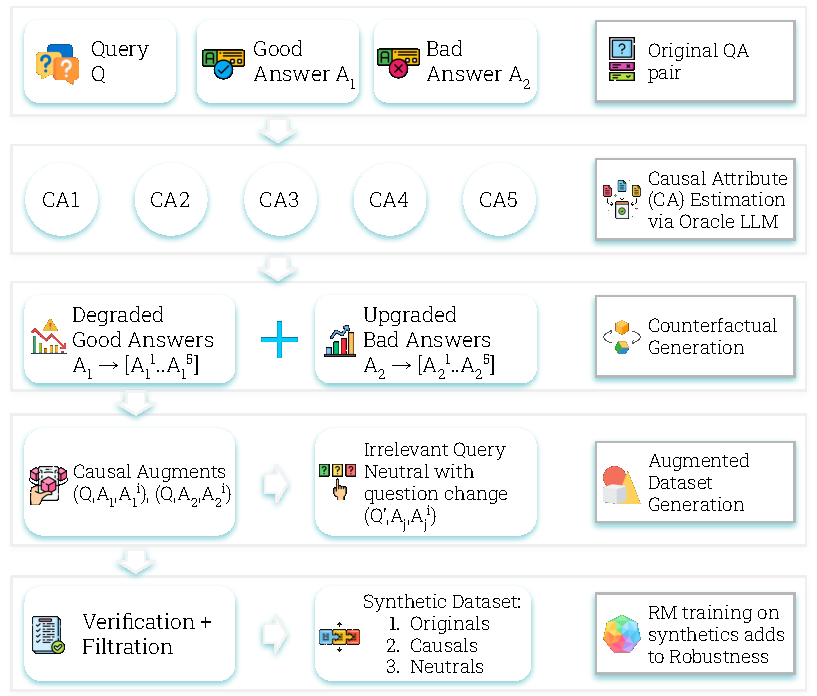
\includegraphics[width=\linewidth]{images/Page1Illustration.pdf}
    \caption{\textbf{The \carma{} Data Augmentation and Training Pipeline.}
From an original QA pair ($\mathrm{Q}, \mathrm{A}_1, \mathrm{A}_2$), an oracle LLM identifies Causal Attributes (CA). This guides counterfactual generation, producing degraded $\mathrm{A}_1$,  
and upgraded $\mathrm{A}_2$ responses.
These form the set of \textit{Causal Augmentations} which teach the model sensitivity to relevant attributes.
Next, we generate \textit{Irrelevant Query Neutrals} by flipping the question on both the newly generated causal contrastive pairs and the original answer pairs, which reduces reliance on spurious correlates.
After verification and filtration, the combined dataset (Originals, Causals, Neutrals) trains the RM, enhancing its robustness.\vspace{-0.5in}}
    \label{fig:enter-label}

\end{wrapfigure}
Attribute-based evaluation, often leveraging LLMs to dynamically generate assessment criteria \citep{gupta2025carmodynamiccriteriageneration}, aims for more grounded reward signals. Other works investigate specific regularization techniques against known biases like length or sycophancy \citep{wang2025beyond}, or explore methods for causal effect estimation like RATE \citep{reber2024rate}.



\vspace{0.1in}
Despite these advances, significant limitations persist. Many approaches target only pre-specified spurious factors, potentially missing unknown correlates, or lack the fine-grained control needed to truly isolate causal quality drivers from confounding spurious features within responses. Augmentation strategies can be coarse \citep{liu2024rrm}, and evaluation-focused methods \citep{gupta2025carmodynamiccriteriageneration, reber2024rate} may not directly equip the RM with mechanisms for robust training against a wide array of spurious variations through targeted counterfactual learning. There is thus a clear need for a framework that systematically leverages a causal understanding of preference formation to train RMs that are both sensitive to causal quality attributes and demonstrably invariant to diverse spurious cues.

\vspace{0.1in}
Motivated by this, we aim to address the following question in this paper:

\vspace{0.1in}
\begin{takeawaybox}
    How do we train reward models to be robust against reward hacking, particularly when a) the specific spurious attributes that an RM may exploit are not known, and b) only the stable or invariant causal attributes found in ground truth/human preferences can be accessed?
\end{takeawaybox}
\vspace{0.1in}

To address this question, we propose \textbf{\carma{}} (Causally Robust Reward Modeling), a novel framework grounded in an explicit causal model of answer generation (Figure \ref{fig:causal_graph}). \carma{} teaches the RM to differentiate genuine quality drivers from superficial cues by augmenting the preference dataset with targeted, LLM-generated counterfactual examples. It creates two key types of synthetic training pairs: (1) \textit{Causal Augmentations}, which introduce changes along specific \textit{causal} attributes (e.g., factuality) to enforce sensitivity to true quality shifts, and (2) \textit{Neutral Augmentations}, using both (i) the causally augmented data as well as (ii) the original preference pairs,
% which reuse the same augmentations as well as the original answer pairs, 
to enforce invariance along \textit{spurious} attributes (e.g., style) using tie-labels. 
Training on this enriched dataset with a modified loss (Section \ref{sec:methodology}) guides the RM towards causal faithfulness. Our evaluations show \carma{} significantly improves robustness, boosting RewardBench accuracy by up to 4.5\%, with substantial gains in Safety and Reasoning.


